\documentclass{article}
\usepackage{graphicx}
\usepackage{float}
\usepackage{amssymb}
\usepackage{amsmath}
\usepackage{mathrsfs}
\usepackage{bm}
\usepackage{mathtools}
\usepackage{fullpage}
\usepackage{wrapfig}
\usepackage{hyperref}

\newcommand{\norm}[1]{\left\lVert#1\right\rVert}

% \DeclareMathOperator*{\argmin}{arg\,min} % thin space, limits underneath in displays
\DeclareMathOperator*{\argmin}{argmin} % no space, limits underneath in displays
% \DeclareMathOperator{\argmin}{arg\,min} % thin space, limits on side in displays
% \DeclareMathOperator{\argmin}{argmin} % no space, limits on side in displays

\begin{document}

\title{Model Outline}
\author{Octav Dragoi}

\maketitle

\section{Introduction}

The problem is stated as a \textbf{molecule optimization} problem: given one molecule, we wish to come up with another one that improves on certain desirable metrics.

The dataset consists of $N$ pairs of molecules from the set of all molecular graphs $\mathcal{G}$, one being the improved version of the other:
\begin{equation}
    \label{eq:problem_setup}
    D = \{(\mathcal{X}_i, \mathcal{Y}_i) : \mathcal{X}_i, \mathcal{Y}_i\in \mathcal{G}, 1\leq i\leq N\}
\end{equation}

Our model will employ the following components:
\begin{itemize}
    \item A \textbf{Graph Convolutional Network (GCN)}, learning Wasserstein node embeddings in $\mathbb{R}^d, d\in \mathbb{N}$. This takes the shape of a parametric function $G$:
    \[G:\mathcal{G} \rightarrow \mathscr{D}_2({\mathbb{R}^d}),\quad G(\mathcal{X})\in \mathbb{R}^{|\mathcal{X}|\times d} \] 
    where $\mathscr{D}_2({\mathbb{R}^d})$ is the space of all finite point clouds in $\mathbb{R}^d$.
    \item A nonparametric \textbf{tangent space embedding} $\phi = \phi_{Z_0}$ taking a reference point cloud $Z_0\in \mathbb{R}^{N\times d}$. This function, described in \cite{kolouri2020wasserstein}, has the form:
    \[\phi : \mathscr{D}_2({\mathbb{R}^d}) \rightarrow \mathbb{R}^{N\times d}\]
    The main reason why we want to use this function is because it generates workable point cloud embeddings in a \textit{fixed size space}, where we can compute our optimization method. This fixes the problem of variable size embeddings, which are harder to parametrize in a neural network. It also allows the use of pointwise translations for optimizing point clouds with the same number of atoms/points.
    \item A pseudoinverse \textbf{decoding function} $F\sim G^{-1}$.
    \[F : \mathscr{D}_2({\mathbb{R}^d})\rightarrow \mathcal{G}\]
\end{itemize}

\section{Training}
Given a graph $\mathcal{X}$, the model should learn an improvement direction $\Delta(\mathcal{X})$. We define this direction as:
\[\Delta(\mathcal{X}_i) = \phi(G(\mathcal{Y}_i))-\phi(G(\mathcal{X}_i)) \]

In other words, we encode the graphs $\mathcal{X}_i, \mathcal{Y}_i$ using the GCN, and then project these encodings onto the tangent space at $Z_0$. The difference between these tangent space vectors contains the information on how to modify one vector to obtain the other, and this is what the model should learn.

The order of the embeddings within $\mathbb{R}^{N\times d}$ is induced by the order we set on $Z_0$, and should not affect the overall modeling process.

\begin{figure}[h!t]
    \label{fig:train}
    \begin{center}
        \includegraphics[page=2,width=\textwidth, trim=0 40cm 0 0 ,clip,angle=0]{images/model_outline_train.png}
        \caption{Training flow. Parametrize $\Delta(\mathcal{X}_i)$ in terms of $\mathcal{X}_i$. Only parametric step is the GCN $G$.}
    \end{center}
\end{figure}

\subsection{Tangent space embedding}

This section discusses a bit more about the embedding function $\phi$, as defined in \cite{kolouri2020wasserstein}. We already exposed the motivation in the introductory part, let us now detail the numerical procedure.

Let $Z_i, |Z_i|=N_i$ be sets of point clouds in $\mathscr{D}_2({\mathbb{R}^d}), 1\leq i\leq M$, and let $Z_0\in \mathscr{D}_2({\mathbb{R}^d}), |Z_0| = N$ be a reference point cloud. Then, we want to view $\phi(Z_i)$ as projections of $Z_i$ on the $\mathscr{D}_2({\mathbb{R}^d})$ manifold's tangent vector space at $Z_0$.

The function $\phi$ is approximated as follows. Let $\pi_i$ be the optimal transport plan between $Z_i$ and $Z_0$, i.e. the solution to the following linear program:
\[\pi_i^* = \argmin_{\pi \in \Pi_i}\sum_{j=1}^N\sum_{k=1}^{N_i}\pi_{jk}\norm{z_j^0 - z_k^i}^2 \]
where $\Pi_i$ is the space of admissible transport plans, i.e.
\[\Pi_i = \left\{\pi\in\mathbb{R}^{N\times N_i}\ \bigg|\ N_i\sum_{j=1}^N\pi_{jk} = N\sum_{k=1}^{N_i}\pi_jk = 1, \forall 1\leq k\leq N_i, 1\leq j\leq N \right\} \]

Then, the Monge map is approximated from the optimal transport plan:
\[F_i = N(\pi_i^*Z_i) \in \mathbb{R}^{N\times d} \]
and the embedding is calculated as:
\[\phi(Z_i) = (F_i-Z_0)/\sqrt{N} \in \mathbb{R}^{N\times d} \]

The function $\phi$ approximates the Wasserstein distance, i.e. $\phi(Z_i) - \phi(Z_0) = W_2(Z_i, Z_0)$ and $\phi(Z_i) - \phi(Z_j) \sim W_2(Z_i, Z_j)$. The quality of this approximation depends on $Z_0$, and therefore $Z_0$ should be picked in an appropriate manner to minimize the error. There is no theoretical bound on the quality of this approximation, though; we will need to check how well it works in practice for our dataset.

\section{Inference}
With the information from $\mathcal{X}$ and $\Delta(\mathcal{X})$, the model should be able to decode $\hat{\mathcal{Y}}$. We define the following:

\[\hat{\mathcal{Y}_i} = F\left(\phi^{-1}\left(\Delta(\mathcal{X}_i) + \phi\left(G(\mathcal{X}_i)\right)\right)\right)\]

Referring to \cite{kolouri2020wasserstein}, $\phi$ is pseudoinvertible, therefore $\phi^{-1}$ should be reasonably well defined. The paper actually uses the inverse in one of their experiments with reasonable success, so it should be suitable for other use cases as well.

\begin{figure}[h!t]
    \label{fig:infer}
    \begin{center}
        \includegraphics[page=2,width=\textwidth, trim=0 40cm 0 0 ,clip,angle=0]{images/model_outline_infer.png}
        \caption{Inference flow. Get the $\Delta(\mathcal{X}_i)$ vector from the trained model, add it to the current embedding and then decode.}
    \end{center}
\end{figure}

\subsection{$F$ discretizer function}

Given a point cloud embedding $Z$, we need a procedure that generates a molecular graph $\hat{Y}$ such that the embedding of $\hat{Y}$ through $G$ is as close as possible to $Z$. The most straightforward way to implement this is by maximizing the likelihood of individual embeddings of nodes and edges.

\[\log P(\hat{Y}|Z) \coloneqq \max_{T}\sum_{i=0}^{N}T_i P(\hat{y}_i = T_i | z_i) + \sum_{i,j=0}^{N} T_{ij}P(\hat{y}_{ij} = T_{ij} | z_i, z_j)\]

This is a starting point, though. We will want to find a way to take into consideration methods of discretizing nodes and edges based on the whole point cloud, not just the individual embeddings.

\section{Open Questions}
\begin{itemize}
    \item The theory around $\phi$ is scarce. How good is the approximation $\phi(X) - \phi(Y)\sim W_2(X,Y)$? How accurate is the pseudoinverse $\phi^{-1}$? Will they be good enough for our purposes?
    \item How to write the decoder $F$? Pani and I have a few ideas, but nothing too clear for now.
    \item How to encode the transition from $\mathcal{X}_i$ to $\mathcal{Y}_i$? The difference between tangent vectors is natural, but maybe we can do something fancier with those vectors.
\end{itemize}

\subsection{Comments and Discussion}

This section is meant for comments and discussion.

\bibliographystyle{ieeetr}
\bibliography{thesisbib}

\end{document}